%First, make the design space as large as possible
% tradeoffs/considerations/selection
% 1 or 2 solutions

%\begin{figure}[t!]
%\centering
%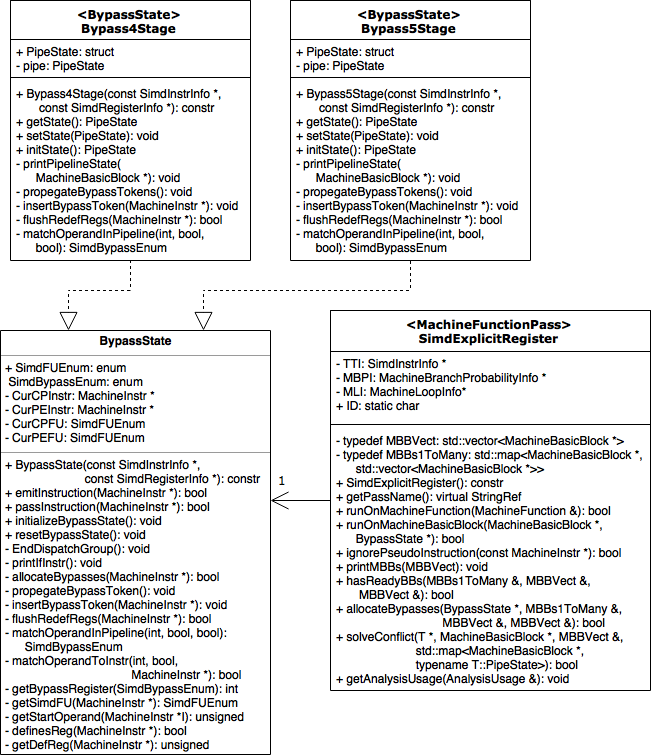
\includegraphics[width=.9\textwidth]{figures/class_diagram}
%\caption{Class diagram of the implemented approach to support explicit datapaths.}
%\label{fig:class_diagram}
%\end{figure}

There is a class called \texttt{BypassState} which should be inherited by each pipeline that we support, e.g. four-stage and five-stage pipeline. It models the values on busses in the bypass network. %It keeps track of values that reside in those busses which keeps track of the . We have This that can be 

\begin{figure}[b!]
\centering
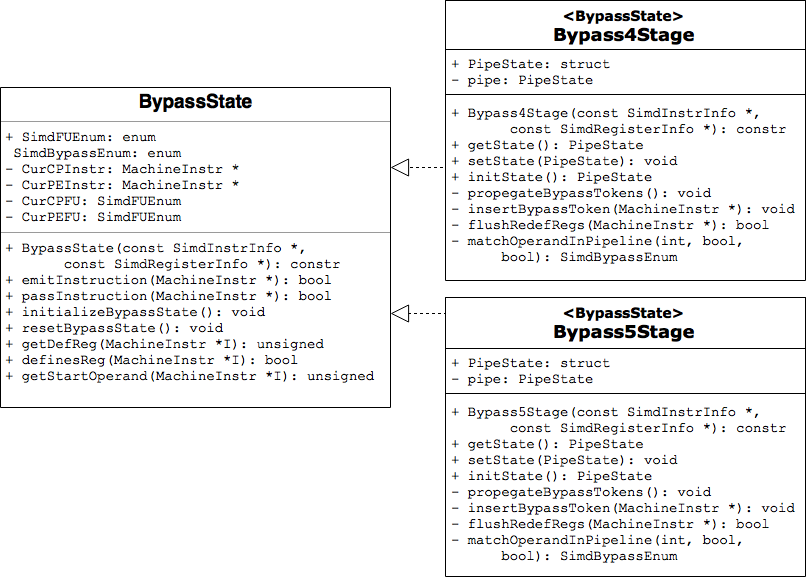
\includegraphics[width=\textwidth]{figures/class_diag_bpstate}
\caption{Class diagram for BypassState, and the inherited classes for the four-stage and five-stage pipelines.}
\label{fig:class_diagram_bpstate}
\end{figure}
%TODO: add following : there was a lot of functionality between the five stage pipeline and four-stage, so we define all shared functionality in \texttt{BypassState}, and stuff specific for a stage in \texttt{BypassXStage}.

We give a class diagram for \texttt{BypassState} in Figure \ref{fig:class_diagram_bpstate}. The classes  \texttt{Bypass4State} and \texttt{Bypass5State} represent the derived classes for the four-stage and five-stage pipeline respectively. Here we use \texttt{insertBypassToken} to pass the instructions in a basic block as tokens to \texttt{BypassState} one at a time and propagate the tokens each cycle using \texttt{propegateBypassTokens}. There is a variable in the derived classes, called \texttt{pipe} which represents the instructions that are currently in our pipeline. The pipeline state can be queried at any giving moment using function \texttt{getState}. This function can be used to acquire the state just before a jump or at the end of a basic block. The functions \texttt{initState} and \texttt{setState} may be used to initialize the state to a empty state, or a given state which is typically done at the beginning of a basic block. We use a function called \texttt{matchOperandInPipeline} to see what bypass can be allocated on a particular use operand of an instruction. It checks whether the operand uses a register defined by any of the instructions the pipeline (by calling \texttt{matchOperandToInstr} and \texttt{getDefReg} for each instruction can be forwarded). In general, it needs to find the newest definition of the register under consideration, therefore, when inserting a bypass token in the pipeline state we remove all occurrences using \texttt{flushRedefRegs}. This way we never have more than one instruction in the pipeline that define the same register, and thus always find the newest definition, if any.

Now lets continue with functions that handle instructions which are used to emit, pass or check an instruction (\texttt{emitInstruction}, \texttt{passInstruction} and \texttt{checkInstruction}). Emitting an instruction consists of the process of specifying which operations are in the current cycle and bypassing their operands according to the current pipeline state. Then pass instruction does the same, but the operands are not bypassed and check instruction does also not actually bypass the operands, but does keep the bypasses that it would allocate in a list. The functions \texttt{allocateBypasses} and \texttt{checkBypasses} do the actual bypassing work by calling \texttt{matchOperandInPipeline} which compares each operand of an instruction to  that can be bypassed. However, there are also flag operands that we do not consider. 
%\lstset{style=customasm}
%TODO: do something cool on the vector slots 
%\vspace{12px}
\begin{lstlisting}
    %loop
        sfgts r2, -64    || v.sfltu   P1, r1, 4
        bf    %loop      || v.slli.P1 r2, r1, 2
        add   r2, r2, -1 || v.add.P1  r7, r6, r2 
    %end:
                         <@\hspace{4px}$\vdots$@>
\end{lstlisting}

%TODO: move next paragraph to above listing, and remove newline
Flag operands occur before register source operands. The code fragment above shows an example of predicate instructions that uses flag operands to either do or not do a certain operation. In this case, we do a shift and add it with something if PE index is smaller than four ($P1$ is true). The function \texttt{getStartOperand} is used to skip flag operands. Alternatively we could also just ignore an operand if it is a flag operand. \\

After each cycle, a call is made to \texttt{EndDispatchGroup} which calls \texttt{insertBypassTokens} for each instruction in the current dispatch (can be two operations, a scalar and a vector op) and propagate the bypass tokens. So to summarize, operands are bypassed when they come across, and at the end of each cycle the pipeline is updated. %Meanwhile using getDef skip all instructions that occur but do not define an instruction. 


%TODO: verify and uncomment
%  later functions do not allocate bypass registers but may be used to insert instructions in the bypass state model, or to check which bypasses would be allocated according to a given bypass state (using \texttt{checkBypasses}), while the first one (\texttt{emitInstruction}) inserts the instruction into the bypass state model and allocates explicit bypasses wherever possible using \texttt{allocateBypasses}.


%TODO: verify and uncomment
% functions \texttt{getDefReg} and \texttt{definesReg} can be used to determine what is written to the register file by an operation, and \texttt{getStartOperand} may be used to see where in an operation we need to start with bypassing RaW dependencies. Function \texttt{matchOperandInPipeline} from the derived classes can be used to see if we can exploit one of the busses in a pipeline. We model these busses with a structure, called \texttt{PipeState}. 

%\begin{table}[b]
%\caption{Representation of struct PipeState.}
%\begin{center}
%\begin{tabular}{@{}l l@{}}
%\toprule
%\textbf{Type} & \textbf{Variable} \\
%MachineInstr* 	& Pipeline[N\_FUNCTION\_UNITS][N\_PACKET\_COUNT][EX\_STAGES]\\
%MachineInstr* 	& WB[N\_PACKET\_COUNT]\\
%SimdFUEnum	& issues[N\_PACKET\_COUNT][EX\_STAGES]\\
%{\small *: pointer}\\
%\bottomrule%%\\
%%{\small * pointer}
%\end{tabular}
%\end{center}
%\label{table:pipe_state}
%\end{table}%